\setcounter{equation}{0}
\chapter{Toughness of double network hydrogels: the role of reduced stress propagation} \label{sec:DoubleNetworks}

\section{Introduction}

While other models have been used to simulate double networks, such as the Multi-spring model used in Ref. \cite{tauber_microscopic_2020} or Molecular dynamics multi-component gels \cite{mugnaiInterspeciesInteractionsDual2025}, they fail to be able to resolve the 


\section{Methodology}
To capture the salient physics of double network materials, we must extend the network model defined in \cref{sec:NetworkStructure} and used in the previous chapters to model both a sacrificial network and a matrix network and how they interact with each other. As a starting point for our model, we again consider a worm-like chain model with Hamiltonian \cref{eq:NetworkHamiltonian}, again only considering the central forces acting on the nodes. We will take each network to evolve almost independently under \cref{eq:NetworkHamiltonian} as in the single network case, again ignoring the volume exclusion principle, both within each network, but also in interactions between the two networks. To connect the two networks, we will consider a subset of nodes in each network to be shared between the two networks, allowing for the two networks to interact via these inter-network connections. These inter-network connections may correspond to either chemically bonded interactions or physical entanglement points between the two networks, and in either case, they enable load sharing, which has been observed experimentally \cite{ahmedBrittleDuctileTransition2014}. Each bond in our system can then be given a modulus $\mu_s$ and $\mu_m$, and a breakage threshold $\lambda_s$ and $\lambda_m$ for the sacrificial and matrix networks, respectively. We will consider a bond to break immediately when its own strain $l/l_0 - 1$ exceeds its corresponding threshold: $\lambda_s$ for sacrificial bonds or $\lambda_m$ for matrix bonds.

In the following work, we consider two forms of network structure, one based on a square lattice (described in \cref{sec:LatticeBasedNetworks} and the other based on Jammed Packing derived networks (described in \cref{sec:PackingBasedNetworks}). The two methods define two ways to construct double network geometries by defining how each network is constructed and how the subset of nodes shared between the two networks is defined. Importantly, they allow us to define a relative length scale difference $M$ between the two networks, which will allow us to capture both the relevant microphysics as well as the macroscopic physics of bulk failure. 

\subsection{Double Lattice Based Networks}
The simplest form of a single network structure is that of a lattice-based network. The Sacrificial network is constructed as described in \cref{sec:LatticeBasedNetworks} by defining a set of lattice vectors and rules for connecting them. The Matrix network can also be generated in the same way, however, with a scaled set of lattice vectors. For simplicity, we choose $M\in\mathbb{Z}$, such that the sacrificial and matrix lattices are commensurate: the matrix lattice vectors are integer multiples of the sacrificial ones. This ensures that the nodes of the Matrix lattice lie exactly on a subset of the nodes of the fine sacrificial lattice. The natural length of each bond $l_0$ is then set in this configuration. The same problems detailed in \cref{sec:LatticeBasedNetworks} occur in double networks, so pruning and perturbing the natural position of each network's nodes. 

While we choose to ignore the volume exclusion principle during the dynamics of the simulation to simplify the forces in our system, only to consider central forces, we can optionally decide to respect this in the network generation steps. This gives us the choice of whether we allow both a matrix and a sacrificial bond to perfectly lie on top of each other in the networks during the network's natural configuration. It's also possible to add further to subdivide the sacrificial bonds such that they connect at every lattice point of the Matrix they pass over. While this would normally give four combinations of lattice network geometries, the case where we do not allow overlaps and do not subdivide the sacrificial bonds decouples the matrix and sacrificial networks, and therefore cannot be considered a double network. An example of the three remaining cases can be seen in \cref{fig:DoubleSquareTypes} for a square lattice with $M=4$.

\begin{figure}[hbt]
    \centering
    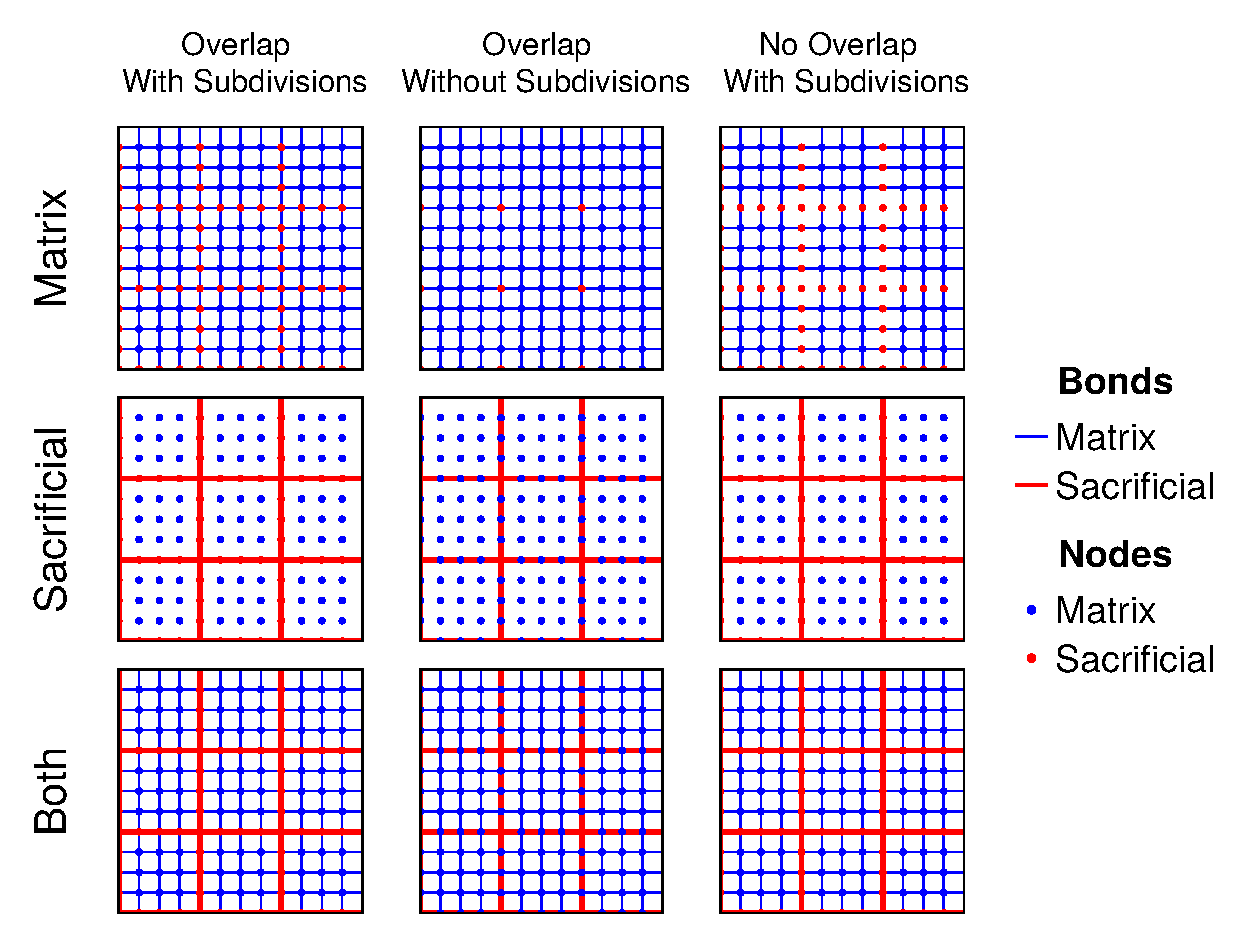
\includegraphics[width=0.75\linewidth]{chapters/DoubleNetworkFracture/NetworkGeneration/SquareTypes-4.pdf}
    \caption{Figure detailing the types of network constructions for a square lattice double network with $M=4$. Each type differs in the choice of nodes which can interact with both the Sacrificial and Matrix networks. In the overlapping network, we ignore the volume exclusion principle and allow both a matrix and a sacrificial bond to co-exist. Networks with Subdivisions subdivide their sacrificial bonds into smaller sections to connect to the Matrix nodes they pass over.}
    \label{fig:DoubleSquareTypes}
\end{figure}

\subsection{Jamming-Based Double Networks}
For jamming-based double networks, we generate the sacrificial network as in the single network case described in \cref{sec:PackingBasedNetworks} through the minimisation of an ensemble of $N_s$ disks of bidispersed radii $R_s$ and $1.4R_s$ in equal numbers at a packing fraction of $\phi = 1.0$. We set the typical length scale of a sacrificial bond by defining the size of our periodic unit cell to be $L_{x0}=L_{y0}=\sqrt{N_s}$ as is done previously. Overlapping pairs of nodes are then connected by a bond with its natural length $l_0$ being set to the distance between the centres of the two disks. The matrix network is constructed similarly, but now starting with an ensemble of $N_m$ disks $R_s$ and $1.4R_s$ in equal numbers at a packing fraction of $\phi = 1.0$, where $R_m \leq R_s$. The ratio of $R_s$ to $R_m$ defines $M = R_s / R_m \in \mathbb{R}_{>0}$, which now takes any positive real value, as by construction the networks do not need to be commensurate to define the internetwork connections. To define the internetwork connections between the sacrificial and matrix networks, we take the existing nodes used to generate the sacrificial network and scale them by a factor of $1/M$ and then pin them to their corresponding node in the sacrificial network, with the remaining $N_m - N_s$ disks randomly initialised. The matrix ensemble is then equilibrated, taking care to ensure that a homogeneous disk distribution is reached despite the inclusions introduced by the pinioned sacrificial disks, with matrix bonds formed in the same manner as in the sacrificial network. The double network can be formed by overlaying the unit cells of the two networks and introducing inter-network connections at all shared nodes, which correspond to all sacrificial nodes by construction.

\begin{figure}[hbt]
\centering
\resizebox{0.9\textwidth}{!}{\begin{tikzpicture}[node distance=1.2cm]

% === Column 1: two stacked boxes ===
\node[draw, line width=1mm, inner sep=0.5\pgflinewidth, minimum width=4cm, minimum height=4cm] (A1) {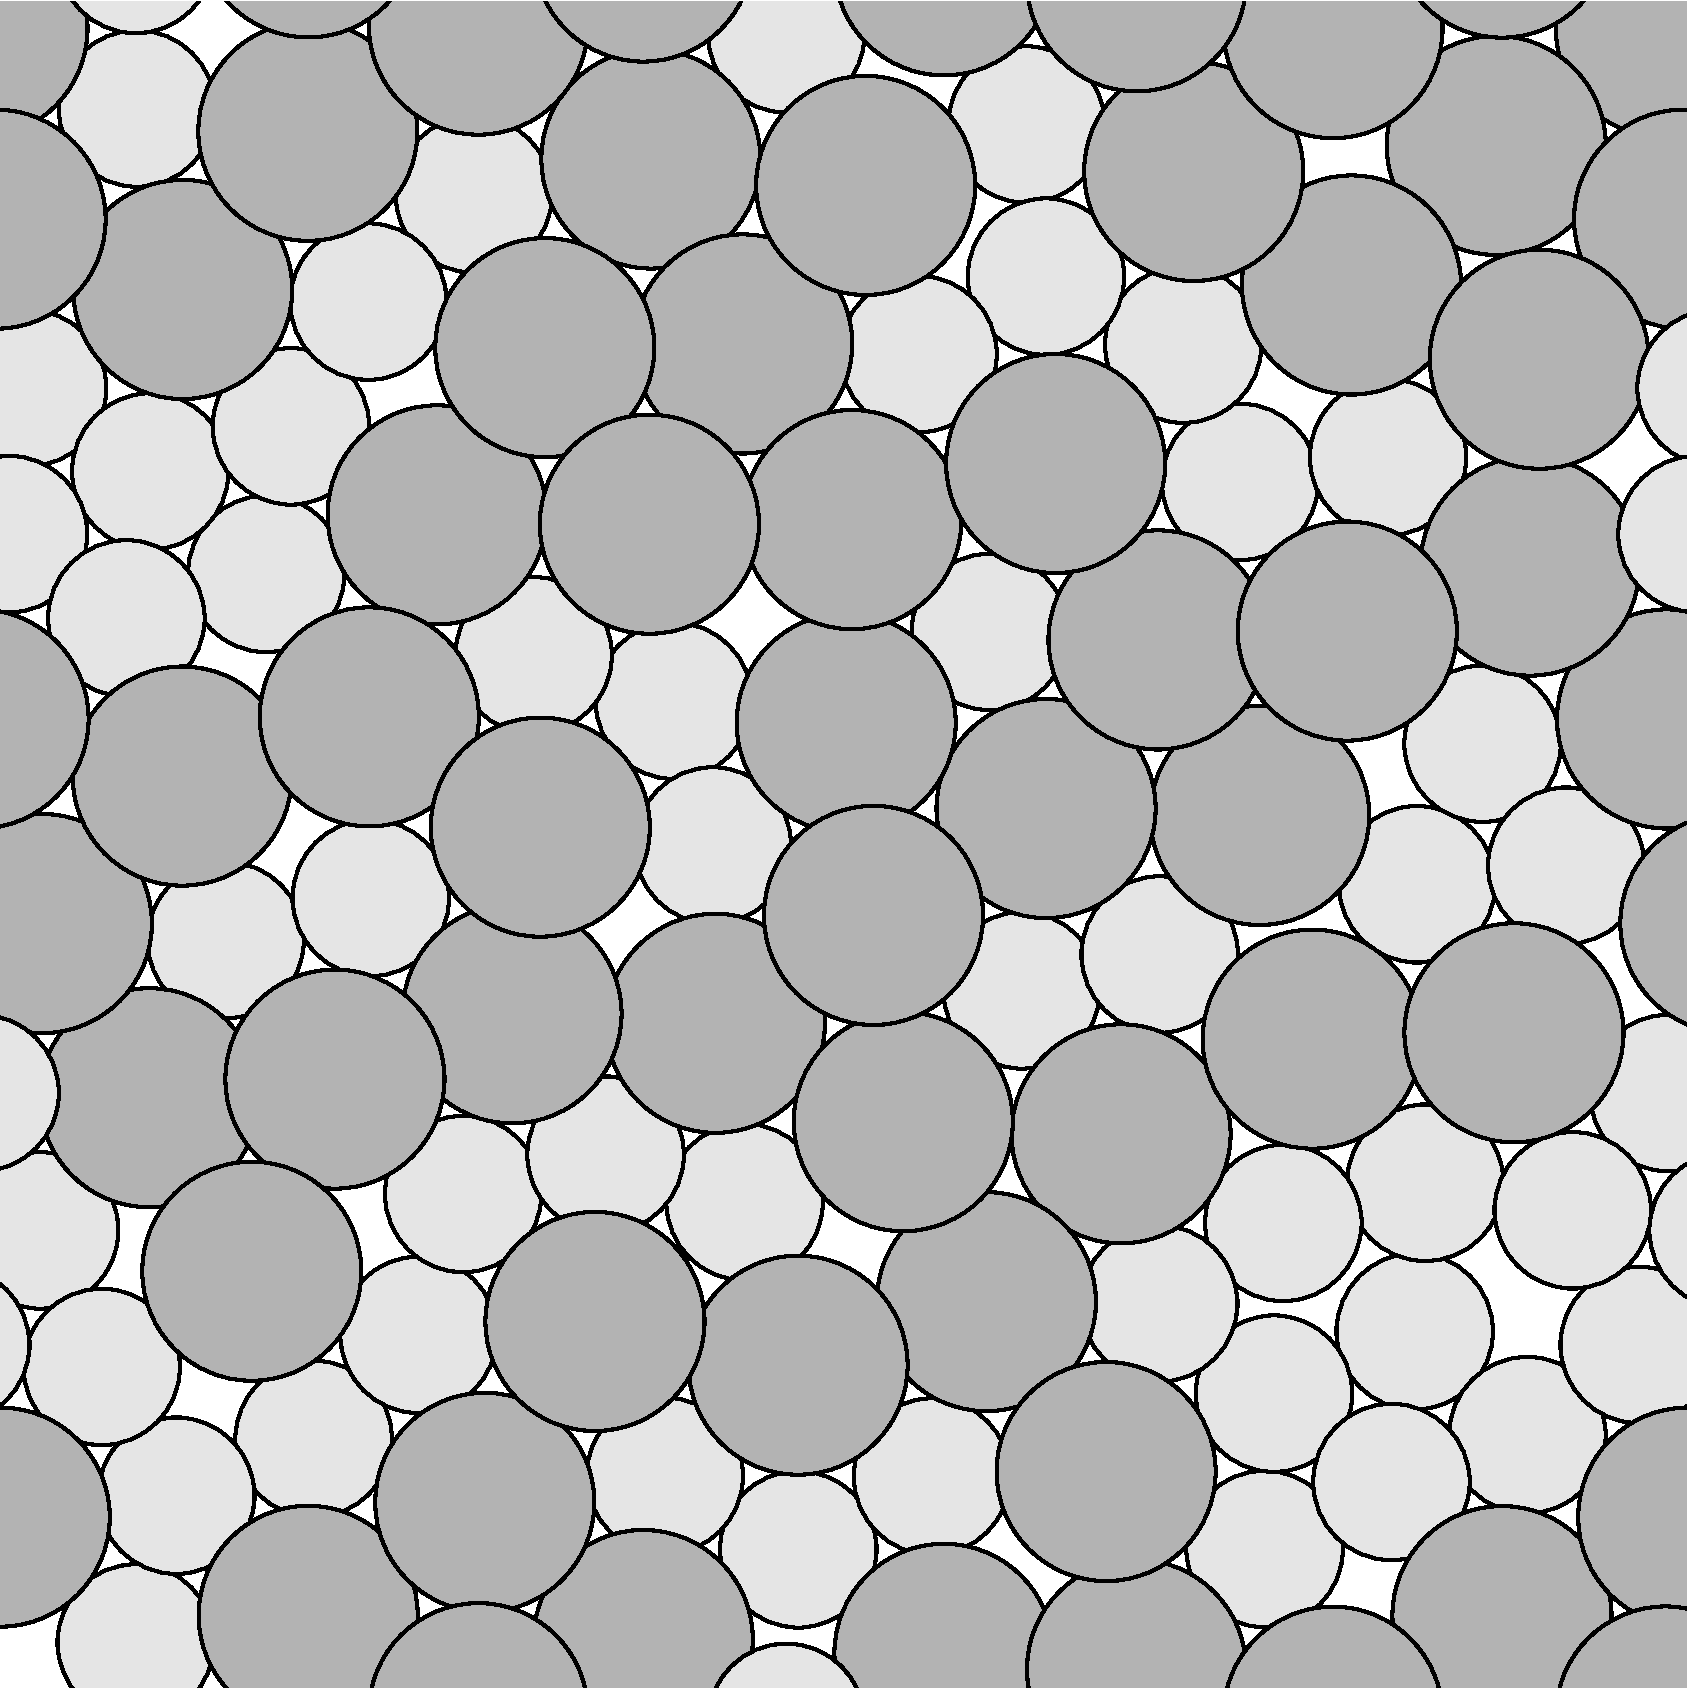
\includegraphics[width=4cm]{chapters/DoubleNetworkFracture/NetworkGeneration/Sacrificial.pdf}};
\node[draw, line width=1mm, inner sep=0.5\pgflinewidth, minimum width=4cm, minimum height=4cm, below=of A1] (A2) {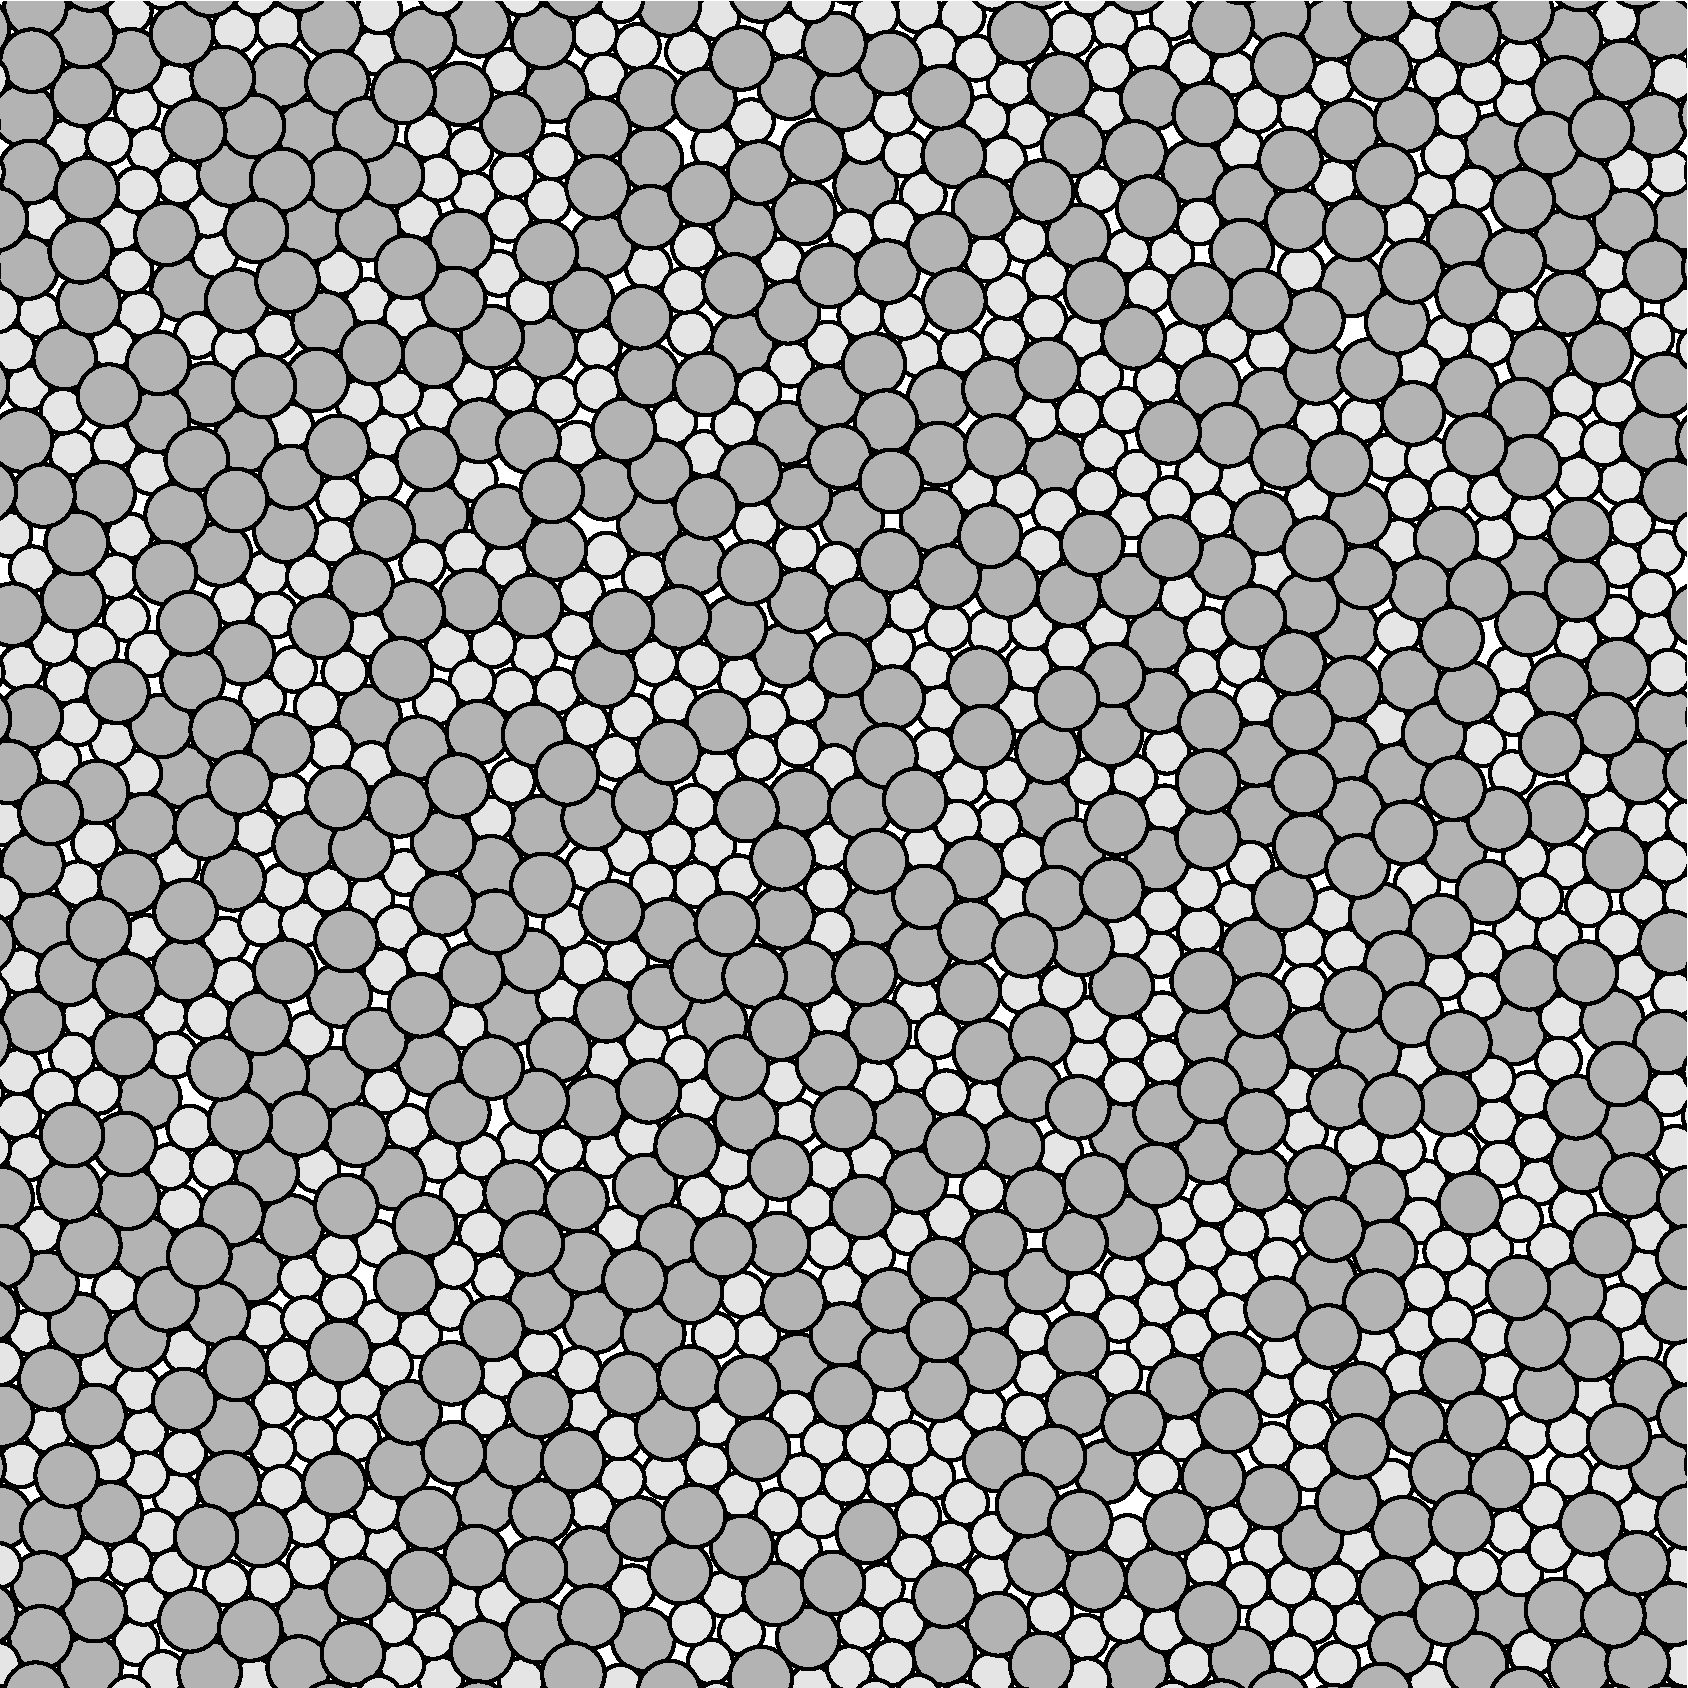
\includegraphics[width=4cm]{chapters/DoubleNetworkFracture/NetworkGeneration/Matrix.pdf}};

% === Column 2: two stacked boxes ===
\node[draw, line width=1mm, inner sep=0.5\pgflinewidth, minimum width=4cm, minimum height=4cm, right=1cm of A1] (B1) {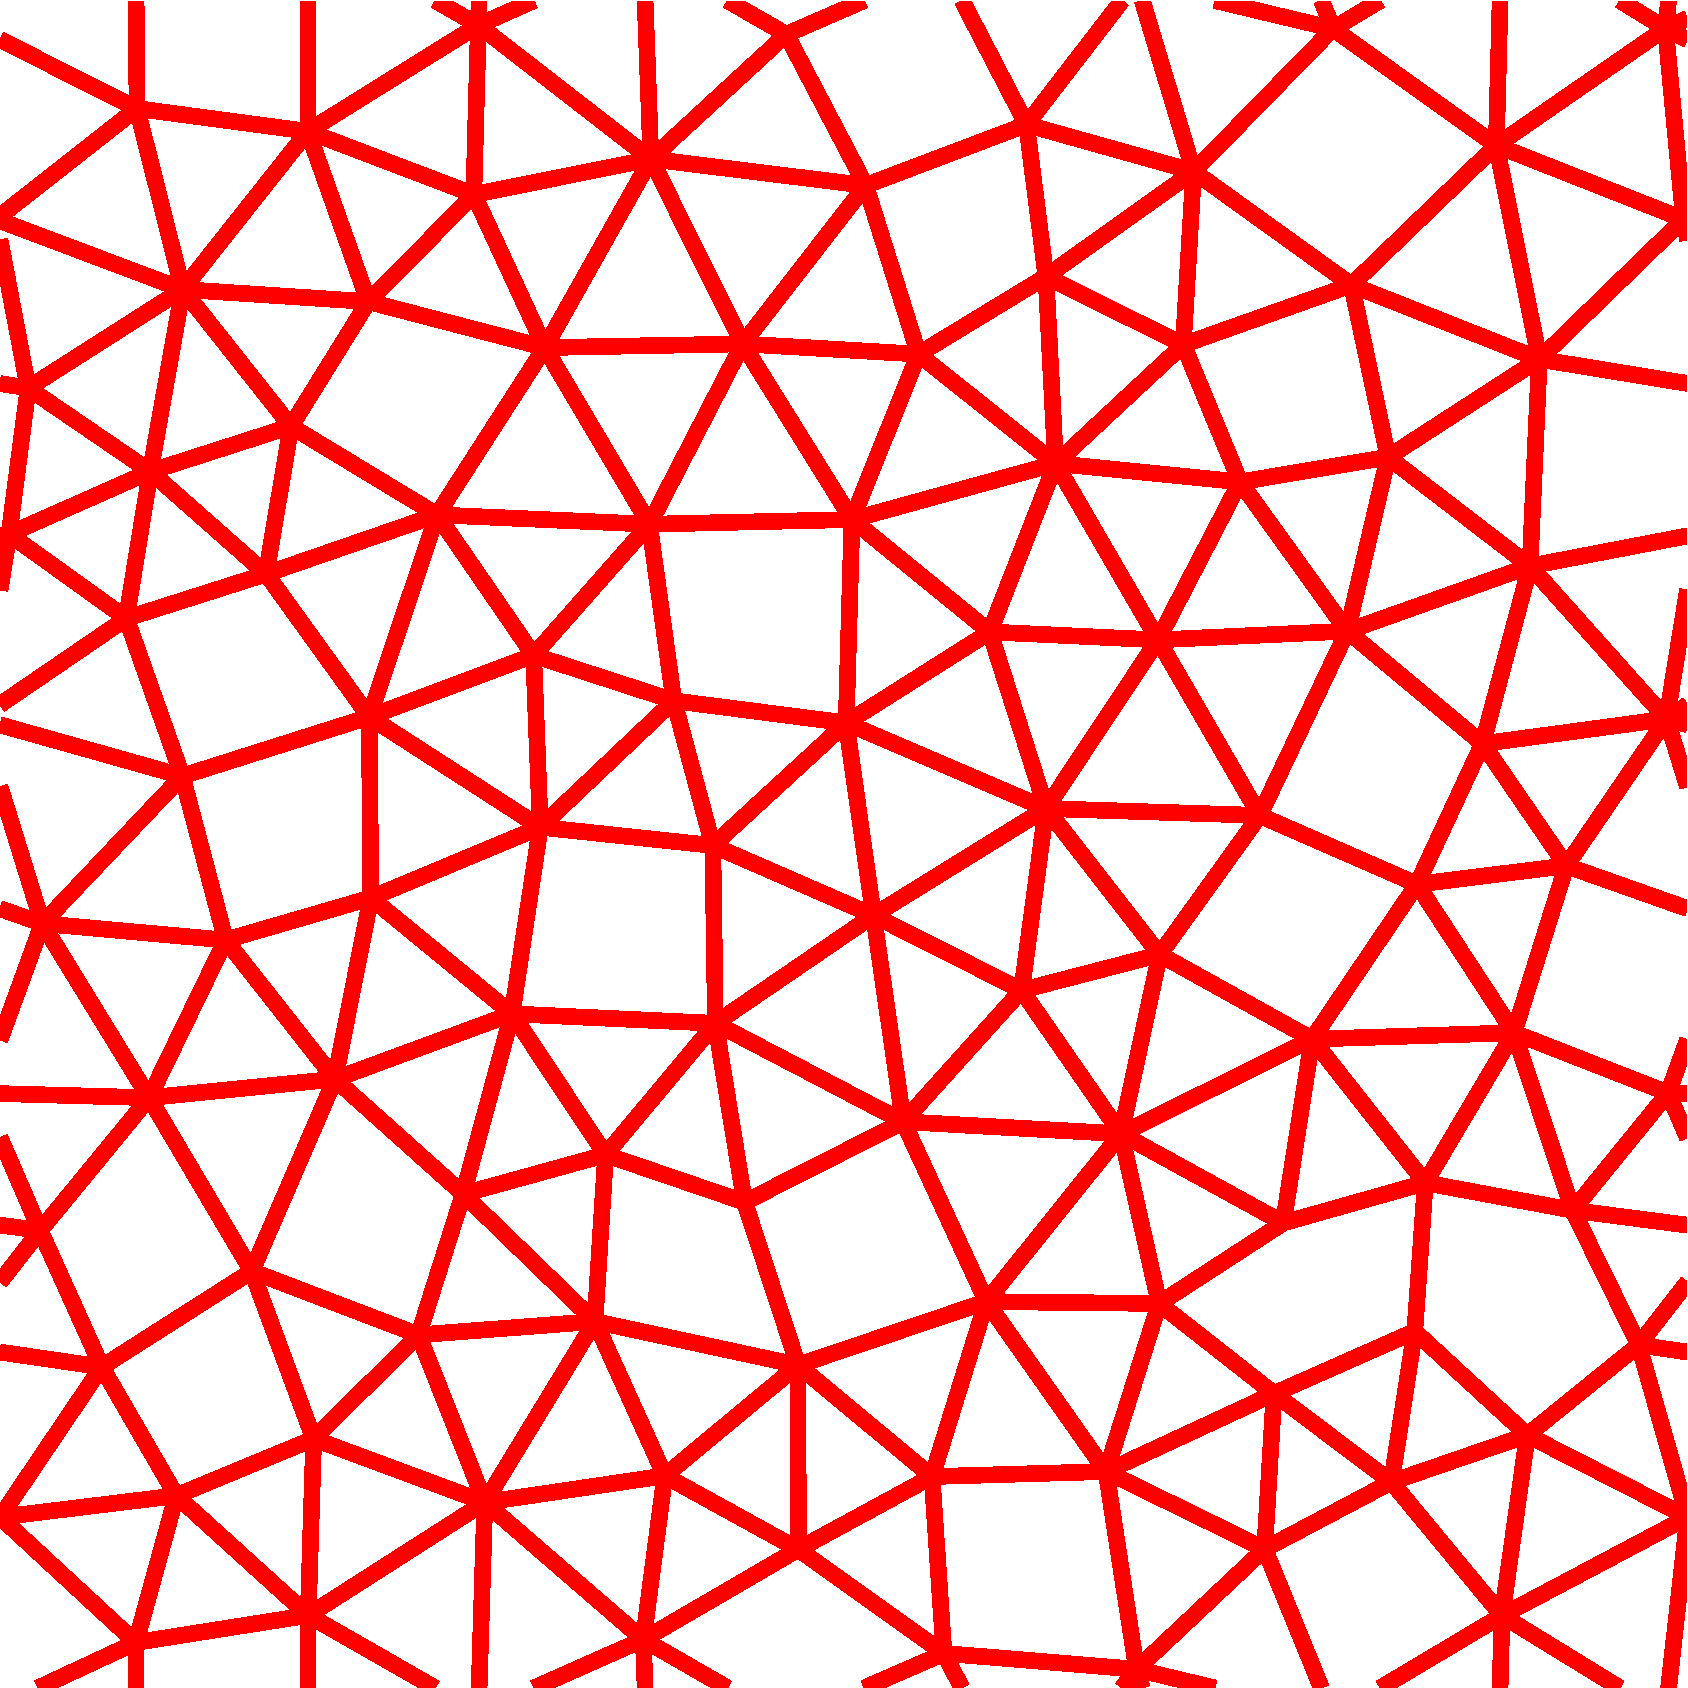
\includegraphics[width=4cm]{chapters/DoubleNetworkFracture/NetworkGeneration/Sacrificial_Red.pdf}};
\node[draw, line width=1mm, inner sep=0.5\pgflinewidth, minimum width=4cm, minimum height=4cm, below=of B1] (B2) {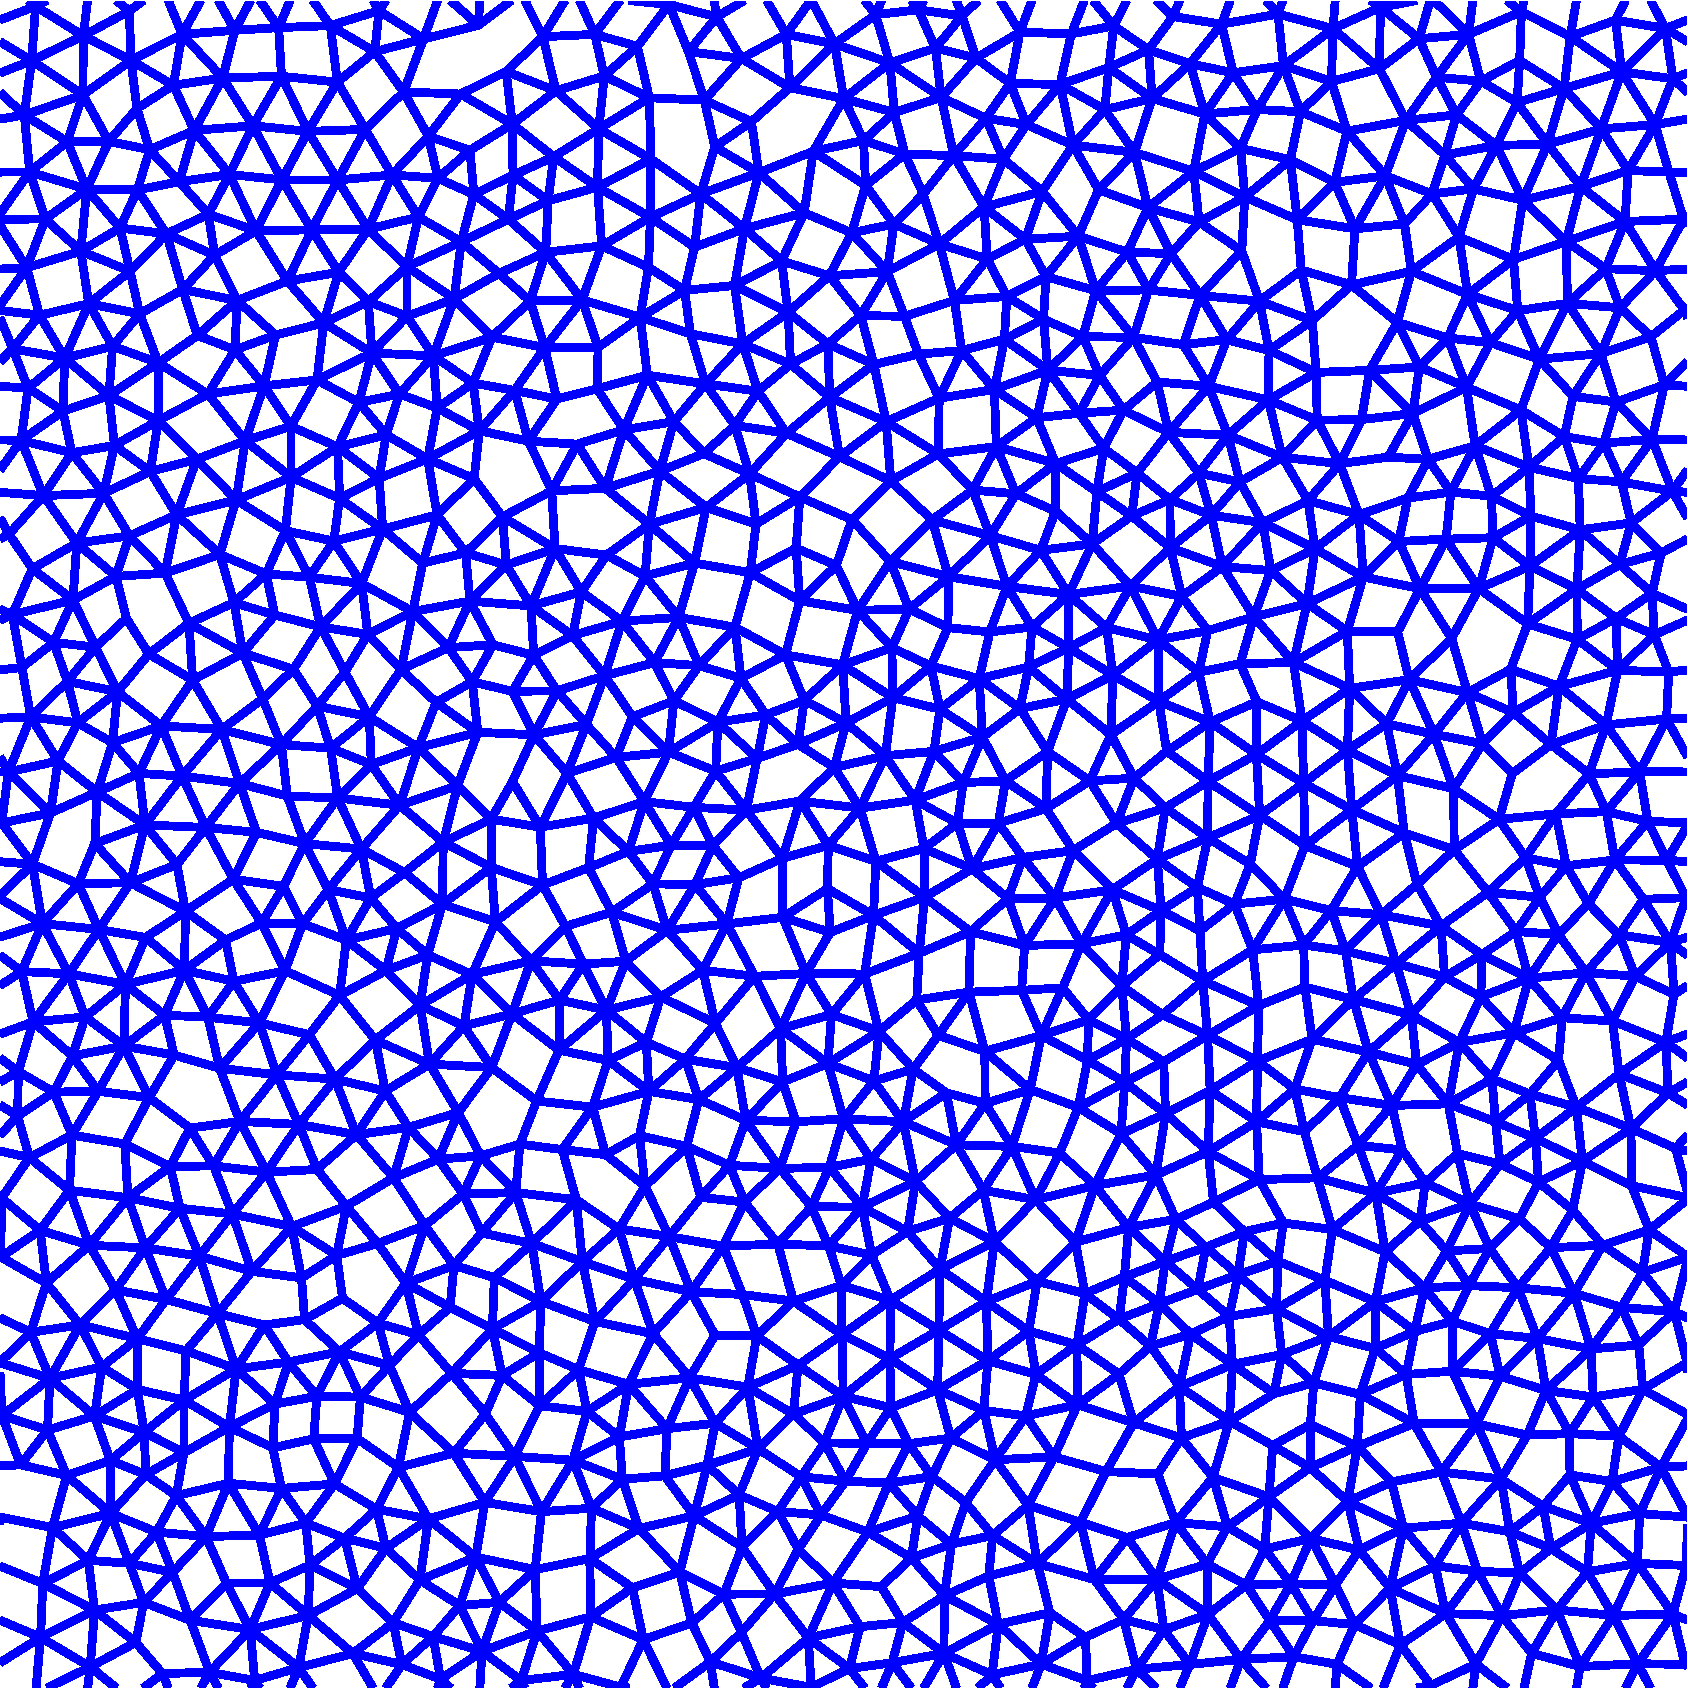
\includegraphics[width=4cm]{chapters/DoubleNetworkFracture/NetworkGeneration/Matrix_Blue.pdf}};

% === Column 3: large single box ===
\node[draw, line width=1mm, inner sep=0.5\pgflinewidth, minimum width=8cm, minimum height=8cm, right=1cm of B1, yshift=-2.8cm] (C1) {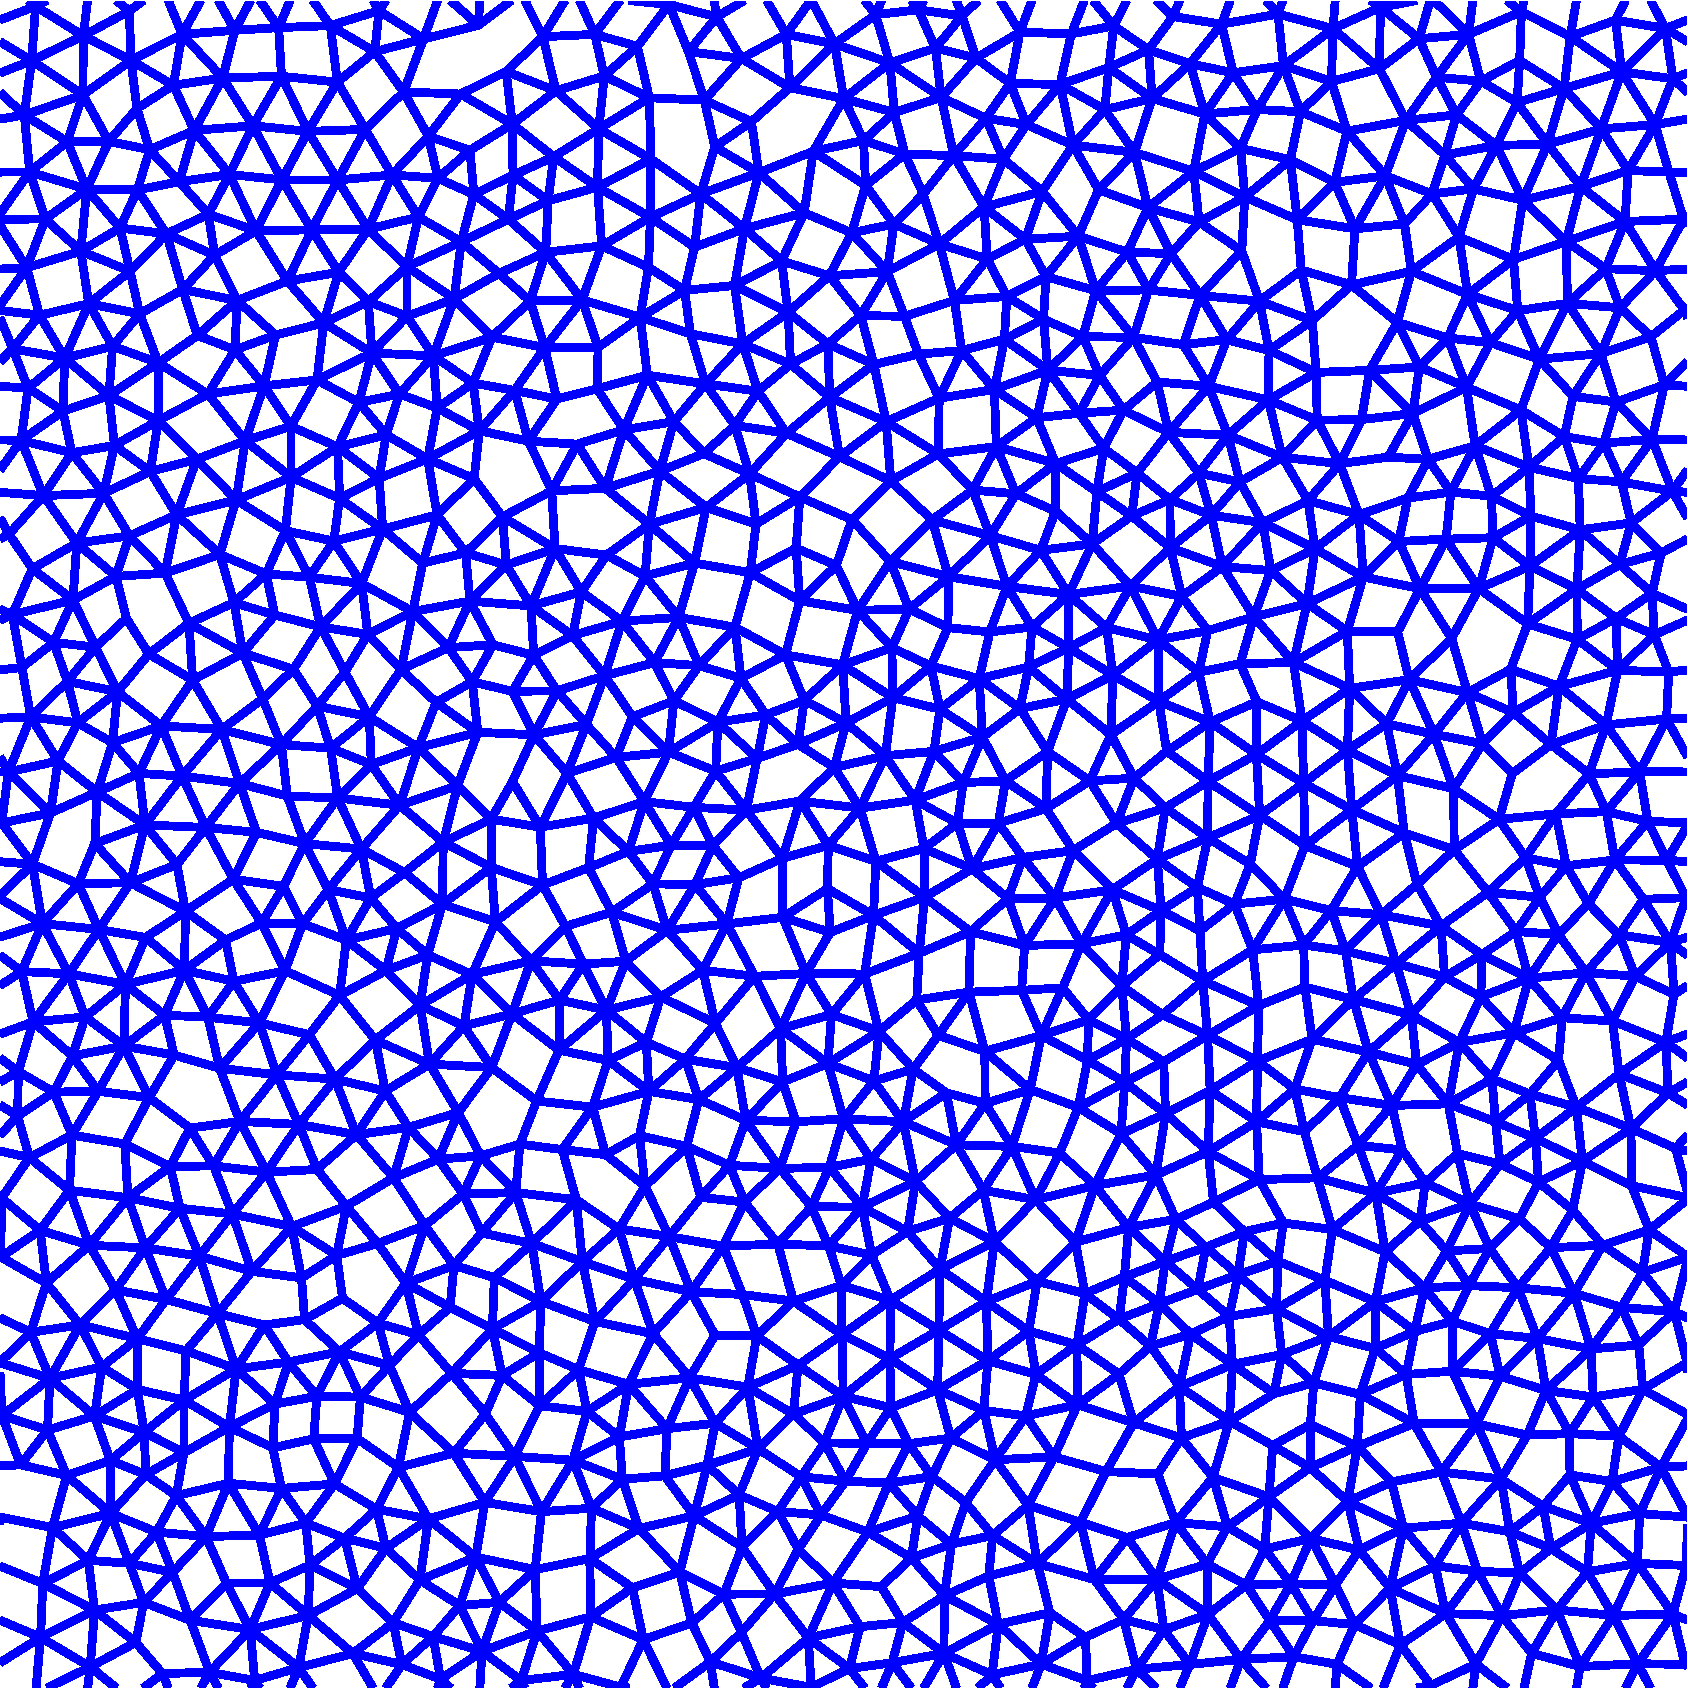
\includegraphics[width=8cm]{chapters/DoubleNetworkFracture/NetworkGeneration/Matrix_Blue.pdf}
};
\node[draw, line width=1mm, inner sep=0.5\pgflinewidth, minimum width=8cm, minimum height=8cm, right=1cm of B1, yshift=-2.8cm] (C1) {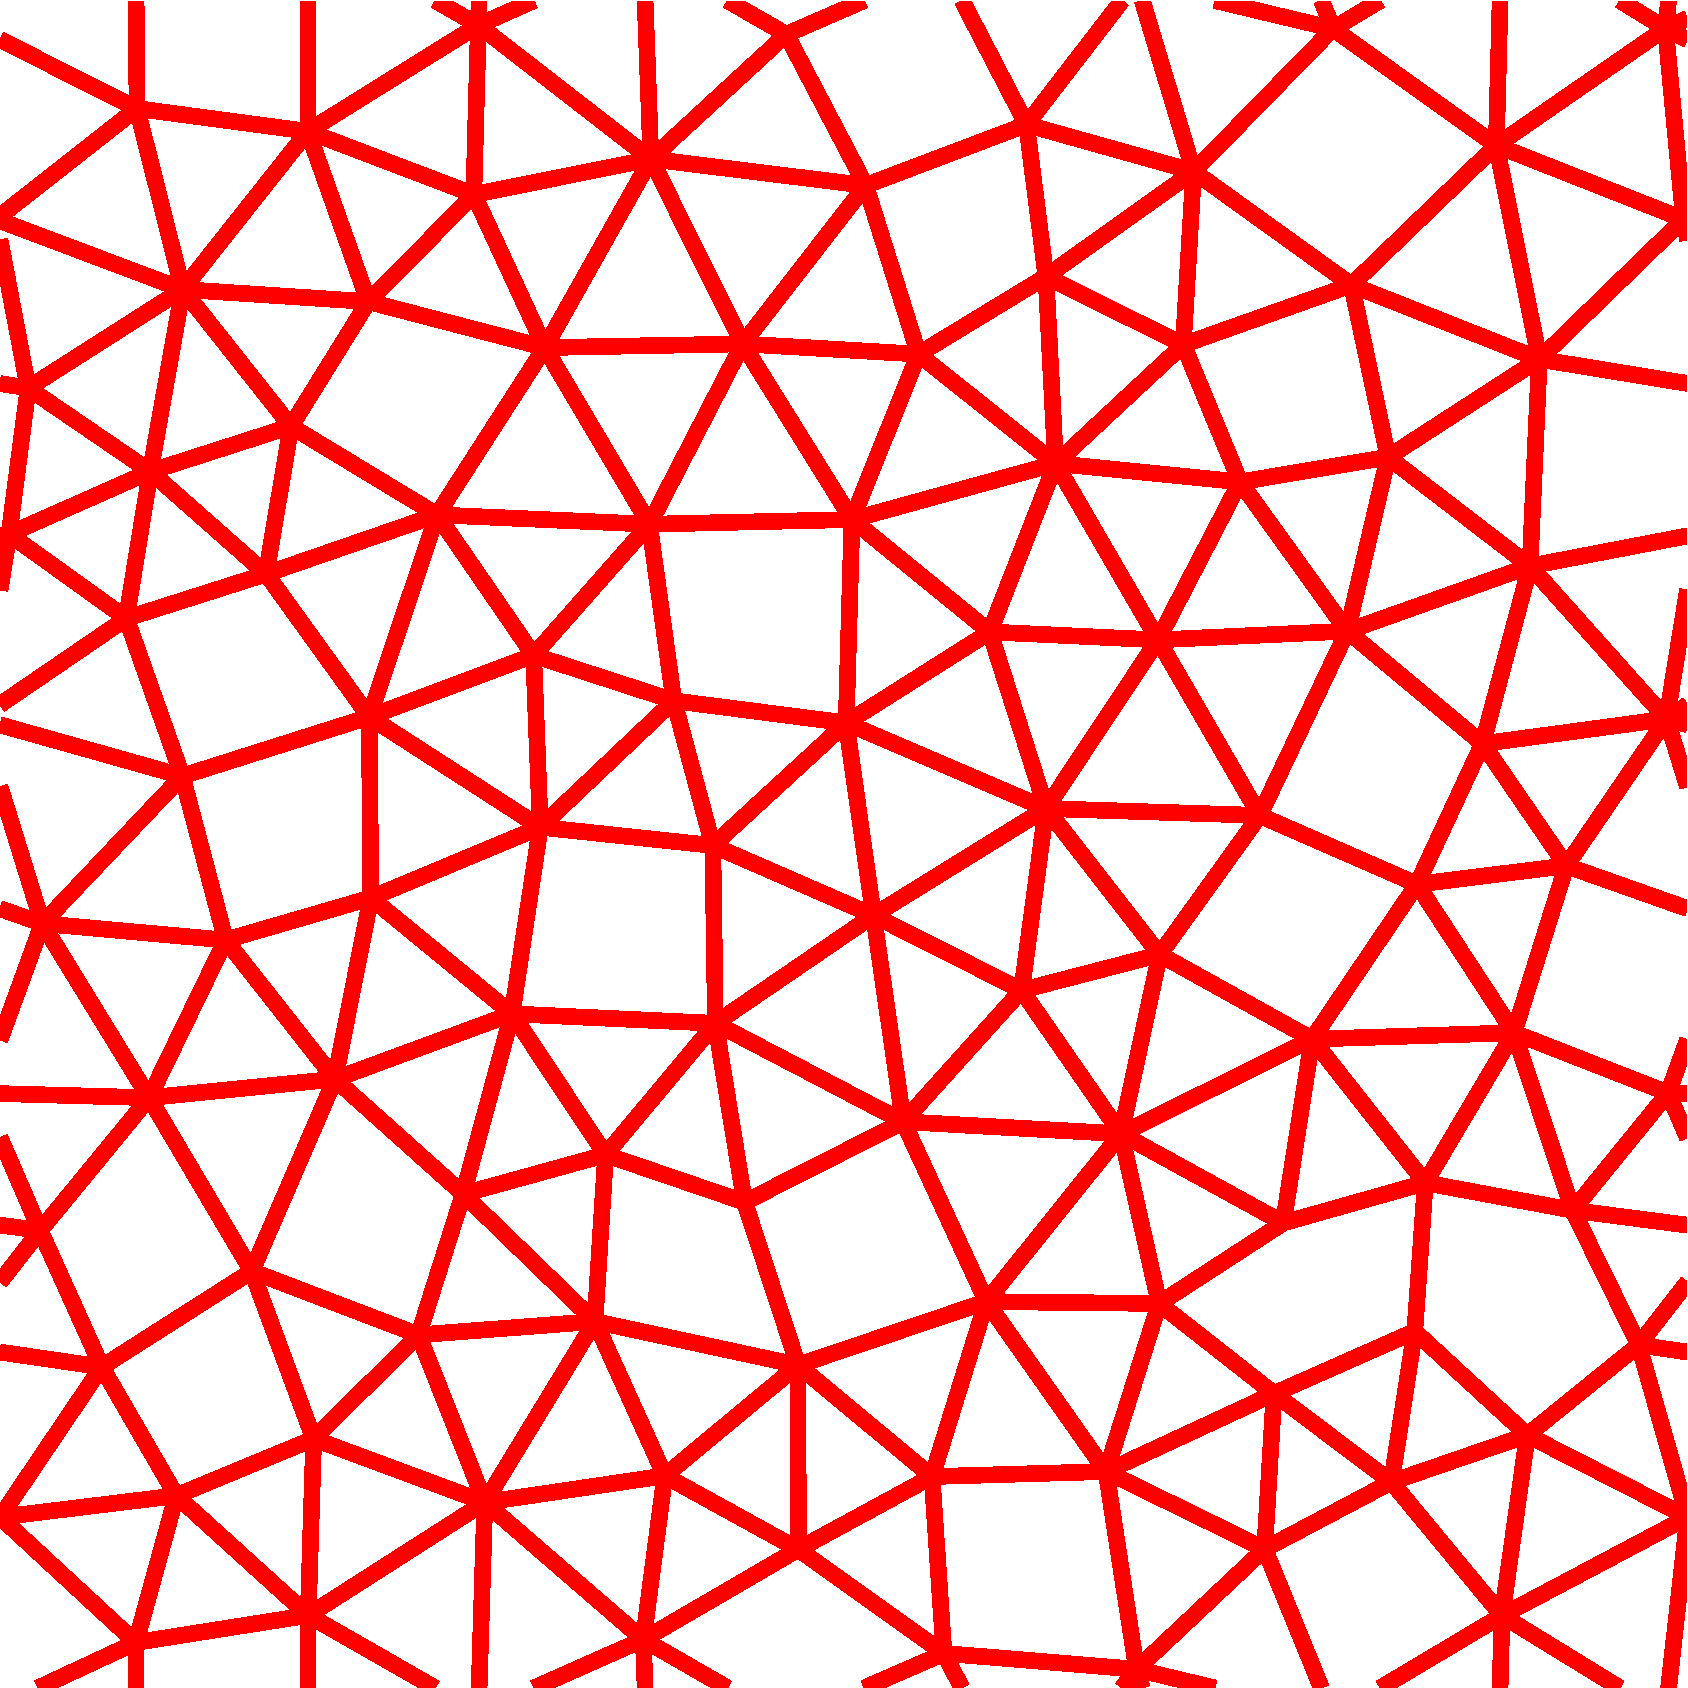
\includegraphics[width=8cm]{chapters/DoubleNetworkFracture/NetworkGeneration/Sacrificial_Red.pdf}
};

% === Arrows Column 1 → Column 2 ===
\draw[->, line width=1mm] (A1.east) -- (B1.west);
\draw[->, line width=1mm] (A2.east) -- (B2.west);

% === Arrows Column 2 → Column 3 ===
\draw[->, line width=1mm] (B1.east) -- (C1.west |- B1.east);
\draw[->, line width=1mm] (B2.east) -- (C1.west |- B2.east);

\end{tikzpicture}}
\caption{Figure detailing how a Jamming-Based Double Network is constructed. The top row illustrates the initial construction of a jammed network as described in \cref{sec:PackingBasedNetworks} through the minimisation of an ensemble of soft disks of two different radii. This gives us the sacrificial network, with bonds shown in red. The bottom row illustrates the construction of the second matrix network again through the minimisation of an ensemble of soft disks of two different radii, however, with pinioned shared disks but rescaled disks from the sacrificial network. This gives a second network with bonds illustrated in blue. These two networks can be combined to form the double network on the right, with inter-network connections at all sacrificial nodes.}
\label{fig:DoubleJammedNetwork}
\end{figure}
    
\section{Rheological Protocol}
Unlike the previous chapter, where we considered systems deformed under simple shear, we consider the system to be subjected to pure shear, with the principal extension axis aligned with the $y$-direction (vertical axis). We deform the square unit cell with initial dimensions $L_{x,0} = L_{x,0}$ along the y-axis and periodic boundary conditions in both axes, preserving the area $L_0^2$ through an effective compression in the $x$-direction. The deformation in the system will be measured by the global engineering strain in the system along the $y$-axis $\epsilon = L_{y}/L_{y,0} - 1$, with the strain rate $\dot{\epsilon}$ considered to be quasi-static, that is $\dot{\epsilon} \to 0$ and the system to be a constant thermodynamic equilibrium. Computationally, this is done by considering steps in the deformation of size $\Delta\epsilon$, which by default are of size $\Delta\epsilon = 10^{-3}$, and for the system to equilibrate with a root mean square (r.m.s.) force on the nodes of magnitude $< 10^{-6}$. 



\section{Paper Images}

\begin{figure}[hbt]
    \centering
    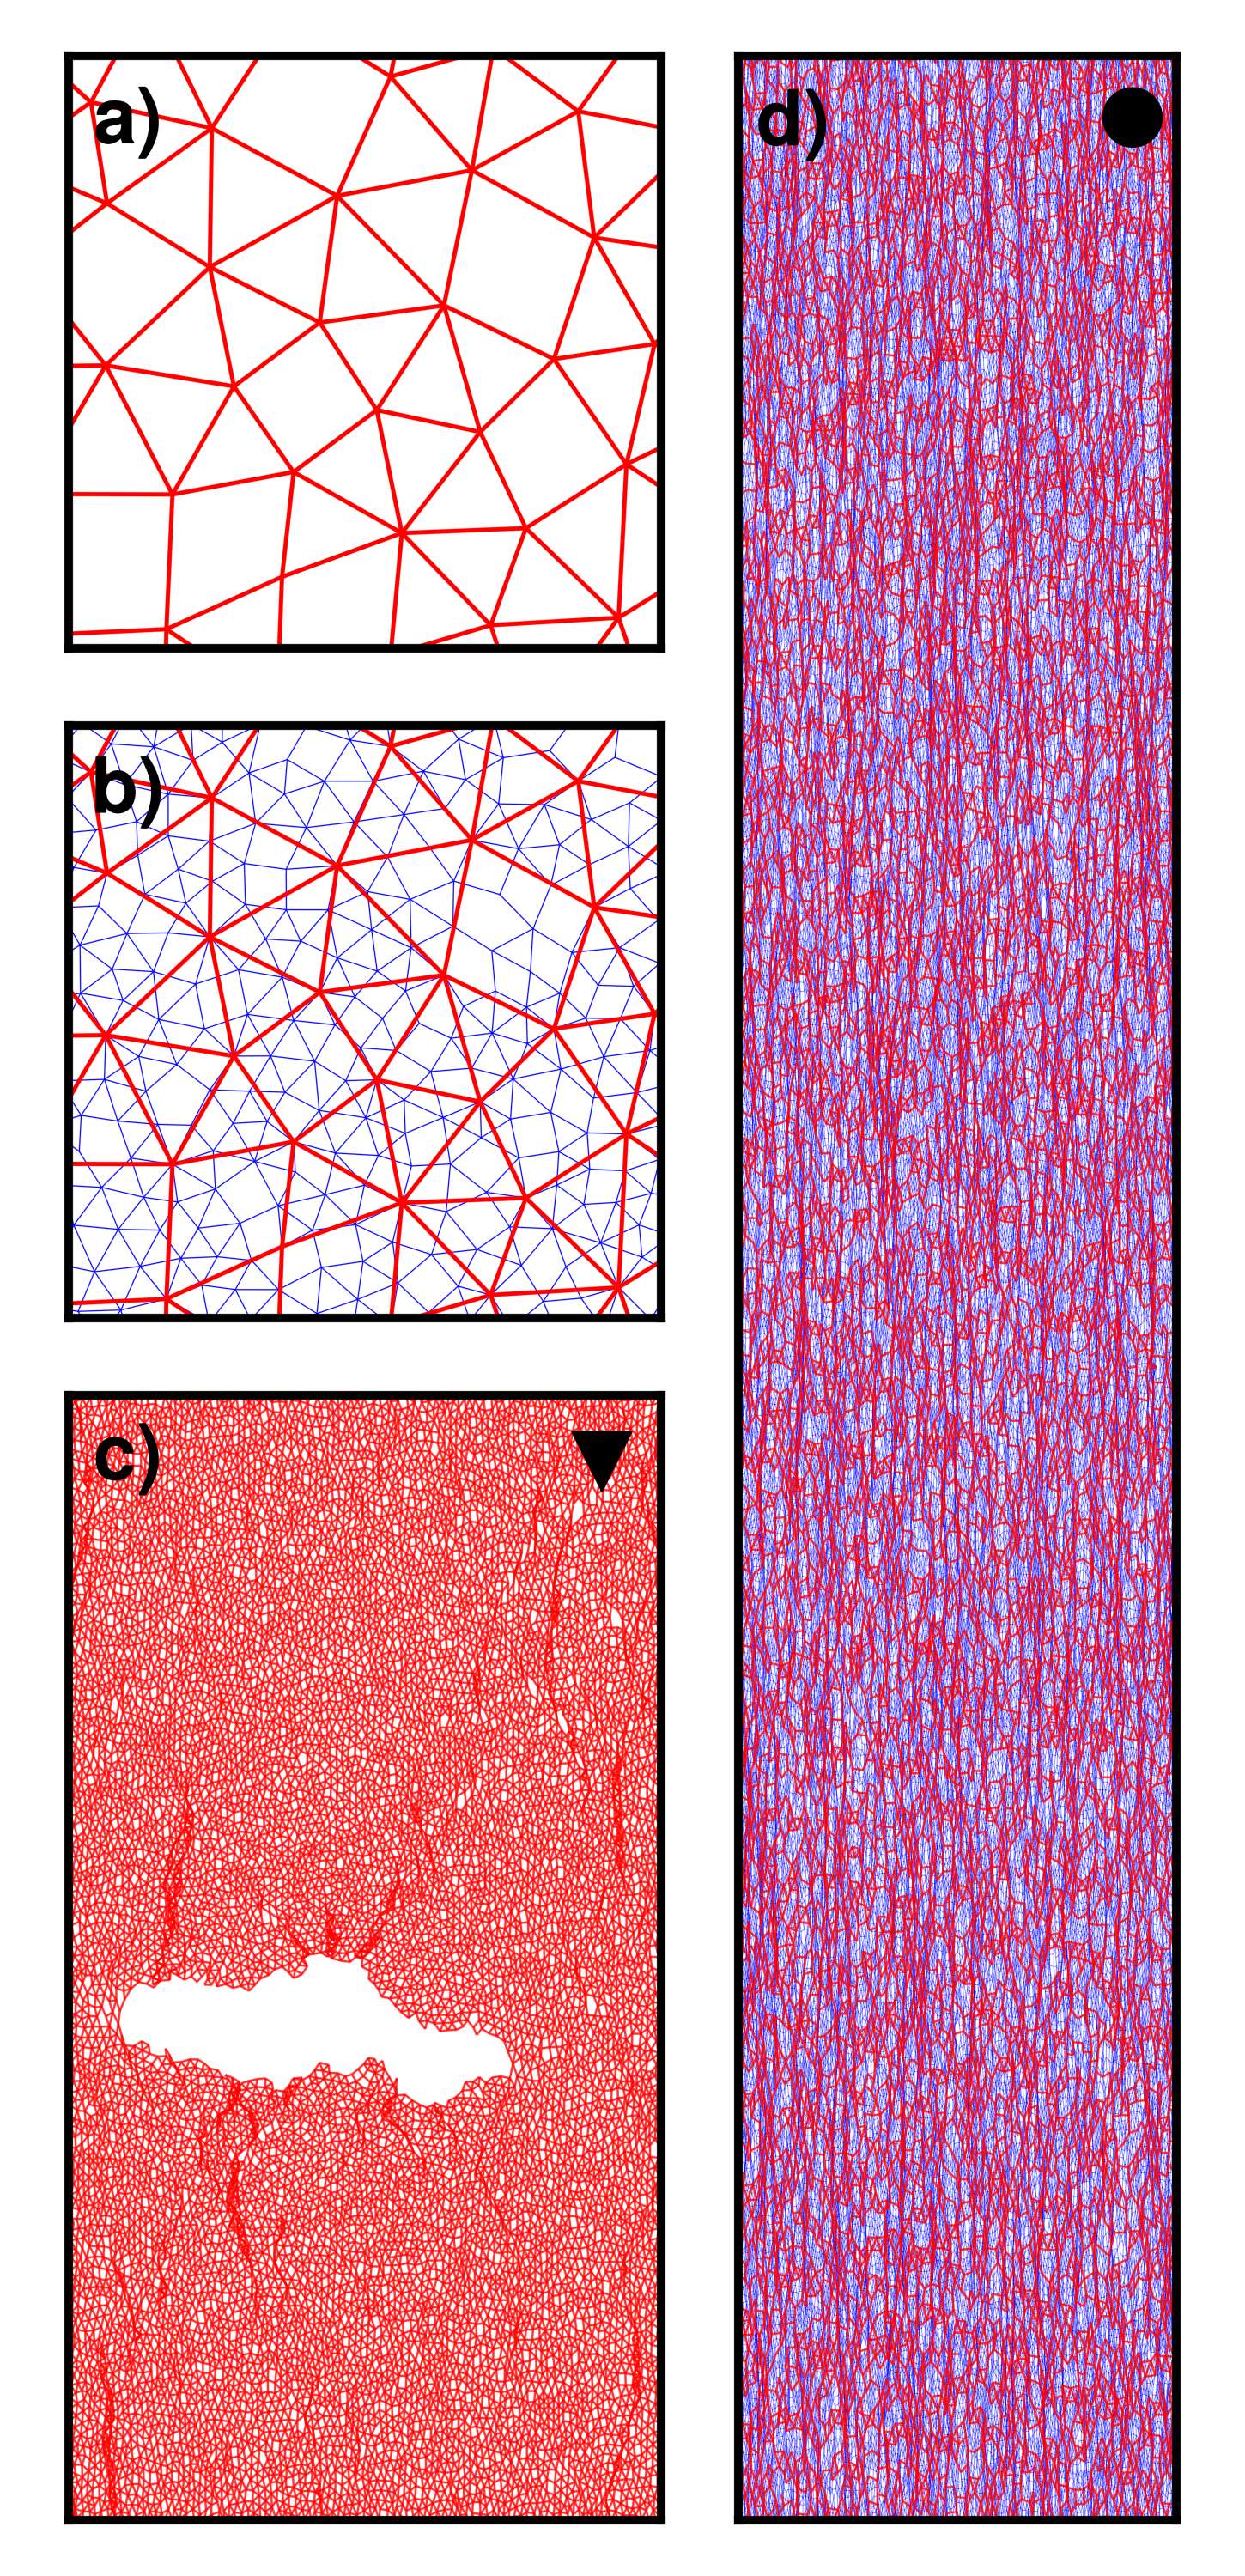
\includegraphics[width=0.7\linewidth]{chapters/DoubleNetworkFracture/Paper Images/Figure1.png}
\caption{Portion of an {\bf a)} single and {\bf b)}  double network, with sacrificial bonds in red and matrix bonds  blue. {\bf c)} Stretched single network at a location on the stress-strain curve shown by the triangle in Fig.~\ref{fig:paperFig2}a). A Macroscopic crack has propagated across the network, causing catastrophic material failure. {\bf d)} Stretched double network at a location on the stress-strain curve shown by the circle in Fig.~\ref{fig:paperFig2}b). Damage has arisen diffusely via many microcracks in the sacrificial network, which do not propagate macroscopically. This allows the double network to stretch much further than the single network without failing.}
\label{fig:paperFig1}
\end{figure}

\begin{itemize}
  \item Is this ok a a whole page figure? Could probably format it to be horizontal, such that it fits nicely along the top and bottom of the page
  \item Do we also generate this for the $z_m=3.5$ case, might be able to make a really nice full page figure if I do this
\end{itemize}

\begin{figure}[hbt]
    \centering
    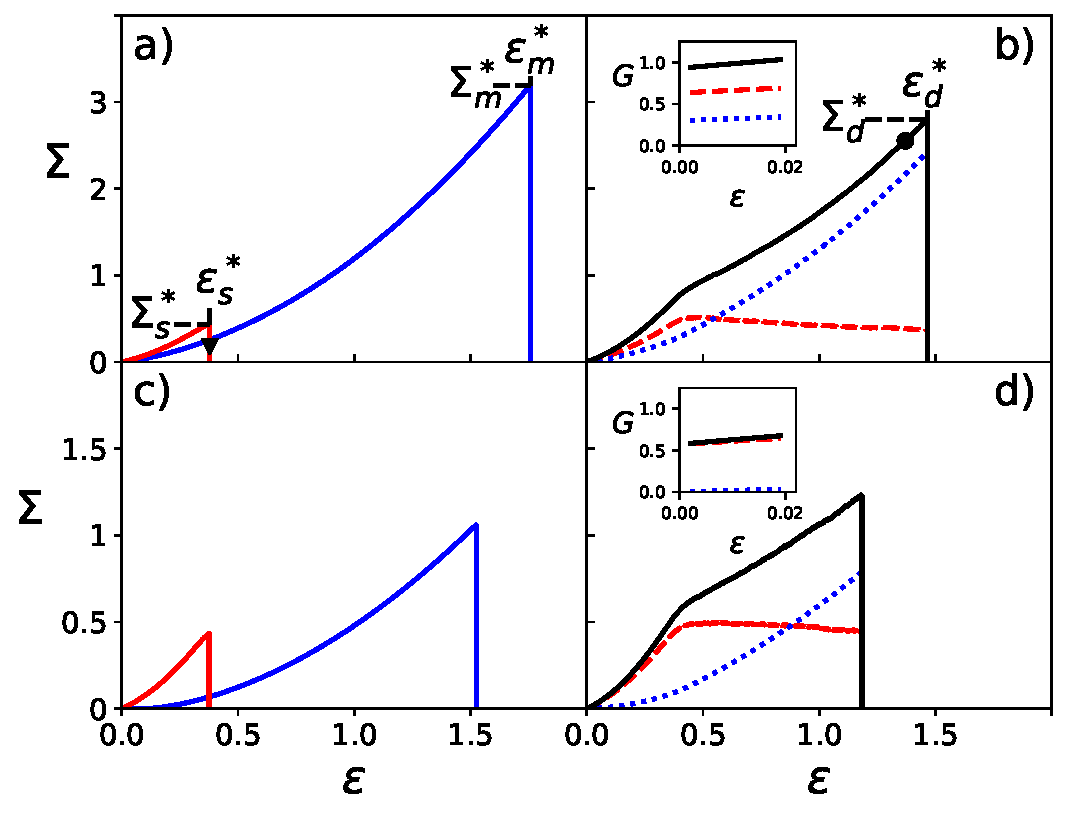
\includegraphics[width=0.5\linewidth]{chapters/DoubleNetworkFracture/Paper Images/Figure2.pdf}
    \caption{Stress-strain curves. {\bf a)} Single sacrificial network (red solid  line) and  single matrix network (blue solid line). {\bf b)} Composite double network (black solid line), with the contributions of the component sacrificial network (red dashed line) and matrix network (blue dotted line) shown separately.  Inset: modulus $G=d\Sigma/d\epsilon$ at small strain. Triangle and circle show the location of the snapshots in Fig.~\ref{fig:network}. Parameters:  $M=3.0,  \mu_m=0.2, \lambda_m=3.0$. {\bf c)} and {\bf d)} show the effect of reducing the matrix network connectivity to $z_{\rm m}=3.5$, as discussed in the penultimate paragraph of the main text.
    }
    \label{fig:paperFig2}
\end{figure}

\begin{itemize}
    \item can definatly make this better formatted for the space
\end{itemize}

\begin{figure}
    \centering
    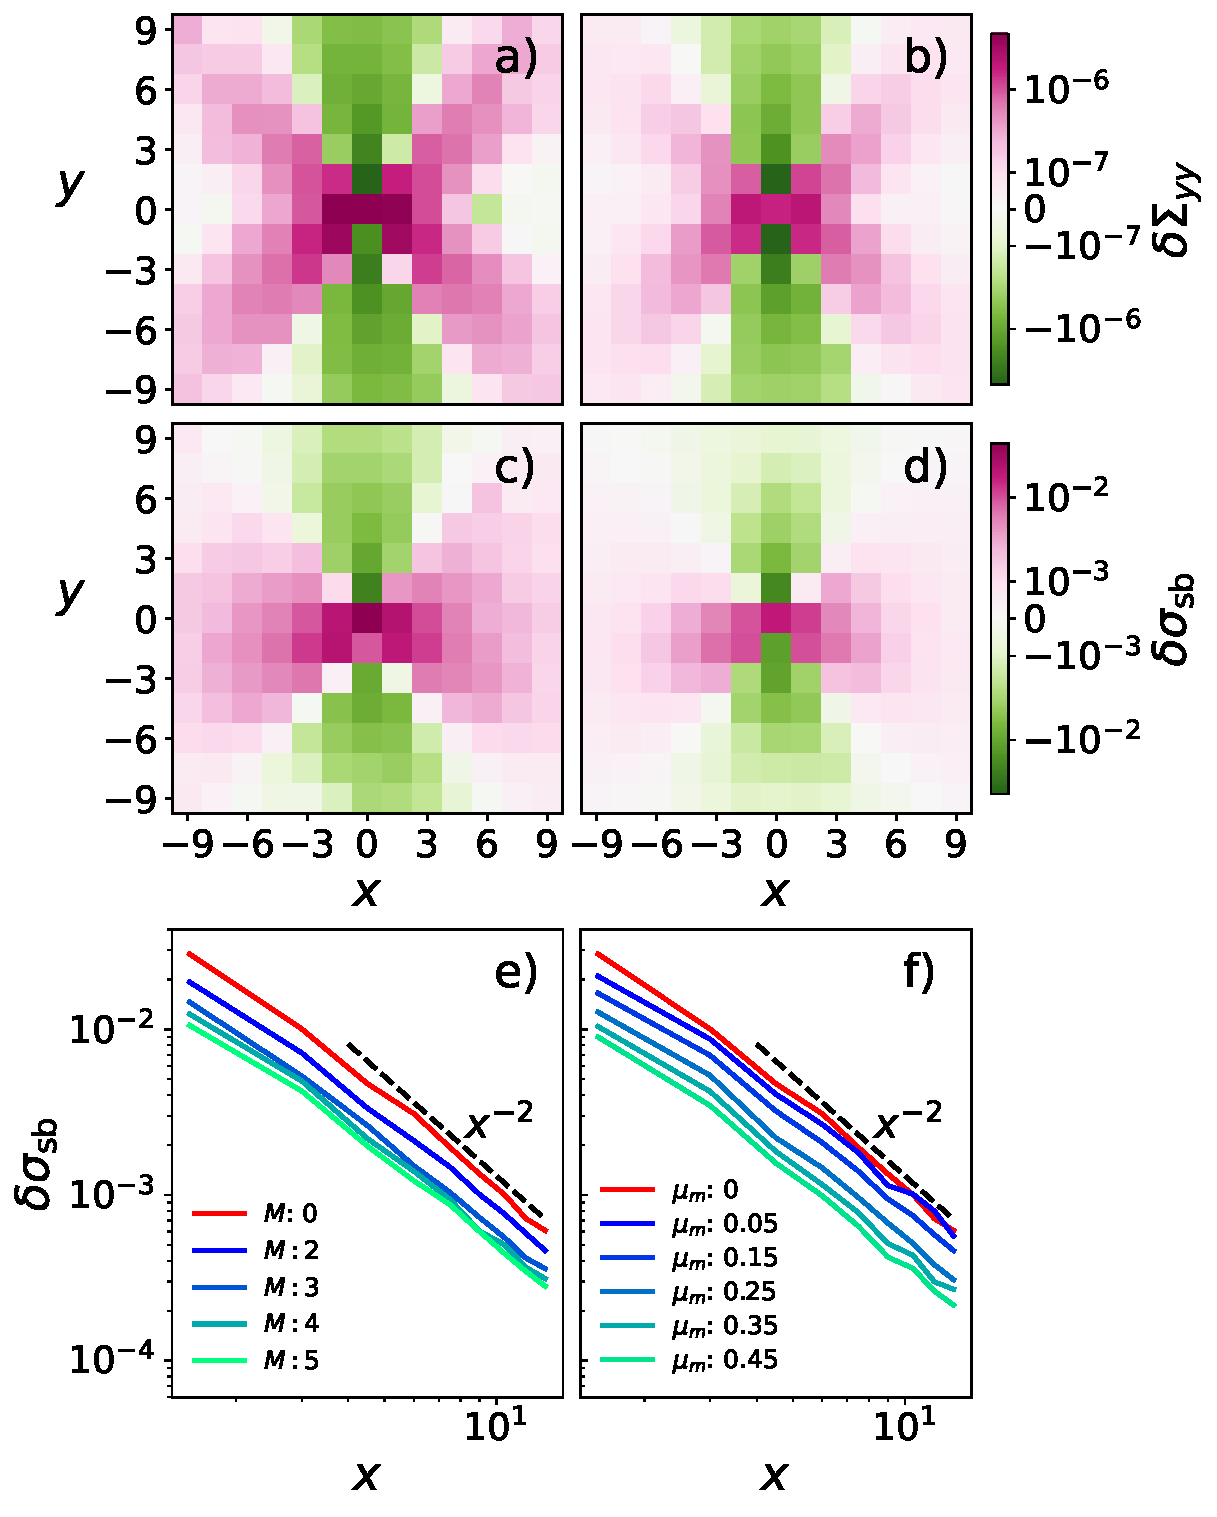
\includegraphics[width=0.5\linewidth]{chapters/DoubleNetworkFracture/Paper Images/Figure3.pdf}
    \caption{Stress propagation to neighbouring sacrificial bonds from the breakage of a sacrificial bond at the origin: (a+c) in a single sacrificial network  and (b+d) in a double network with $M=5.0, \mu_m=0.2$.  Colourscales show the change due to stress propagation of (a+b)  the $yy$ component  of the Kirkwood stress  $\delta\Sigma_{yy}$; and (c+d)  the sacrificial bond stress  $\delta\sigma_{\rm sb}$, with $\sigma_{\rm sb}\equiv \mu_s(l-l_0)/l_0$. Each quantity is averaged over all bonds at each grid square. e+f) show the change in bond stress as a function of distance along $x$  at $y=0$ for e) several $M$ at fixed $\mu_m=0.2$, and f) several $\mu_m$ at fixed $M=3.0$.  
Lengths are expressed in units such that $\Delta x=1$ corresponds to the typical sacrificial bond length. The propagator of a single sacrificial network is recovered for $M=0$ or $\mu_m = 0$. }
    \label{fig:paperFig3}
\end{figure}

\begin{itemize}
    \item really like this figure, in particular the top 4
    \item seperate into two figure, top 4 and bottom four
    \item We may be able to show more cases, with a change in $M$
    \item Do we do the same as a fn of $\mu_m$, i.e have a grid for each of e) and f)
\end{itemize}

\begin{figure}
    \centering
    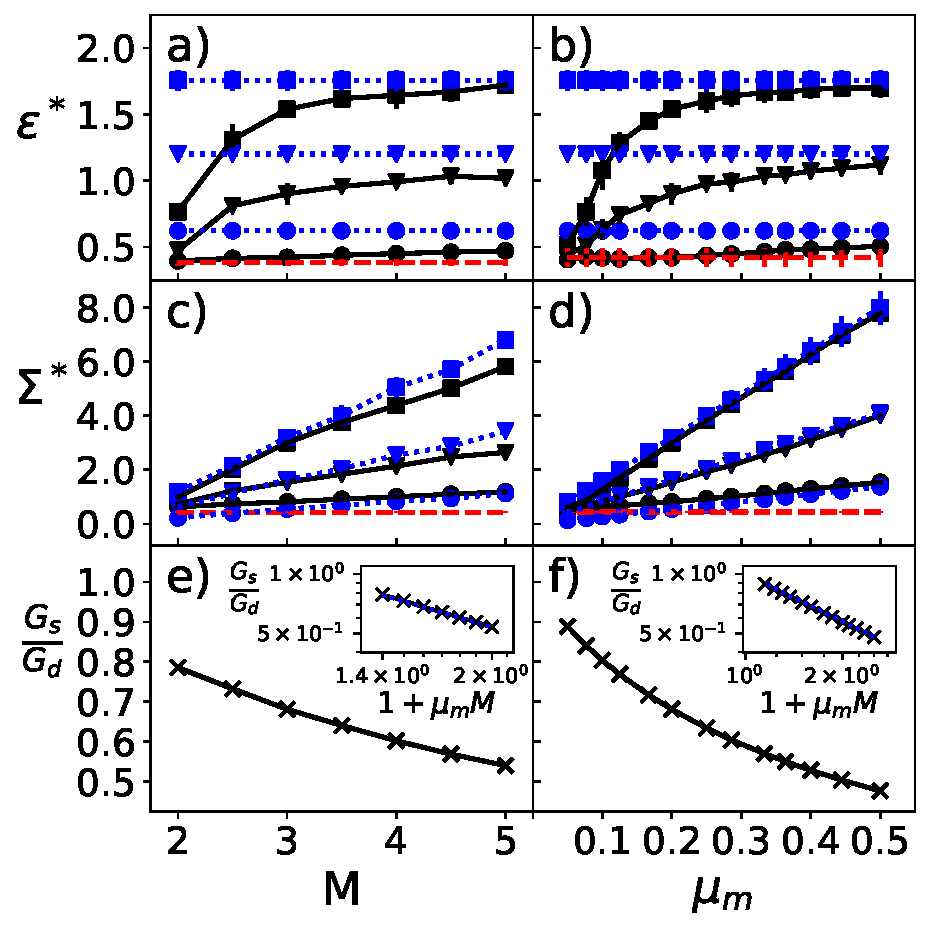
\includegraphics[width=0.5\linewidth]{chapters/DoubleNetworkFracture/Paper Images/Figure4.pdf}
    \caption{{\bf Top:} failure strain of double network (black solid lines) as a function of a) the amount of matrix $M$  and b) matrix bond stiffness $\mu_m$, shown in each case for matrix bond breakage thresholds $\lambda_m=1.0, 2.0, 3.0$ in curves bottom to top, marked by circles, triangles and squares respectively.  Failure strains of the corresponding single sacrificial network and single matrix network are shown by red dashed and blue dotted lines respectively. {\bf Middle:} as in a+b) but now showing failure stresses. {\bf Bottom:} modulus of the sacrificial network relative to that of the double network. Matrix bond stiffness $\mu_m=0.2$ in a,c,e). Amount of matrix $M=3.0$ in b,d,f).}
\end{figure}

\begin{figure}
    \centering
    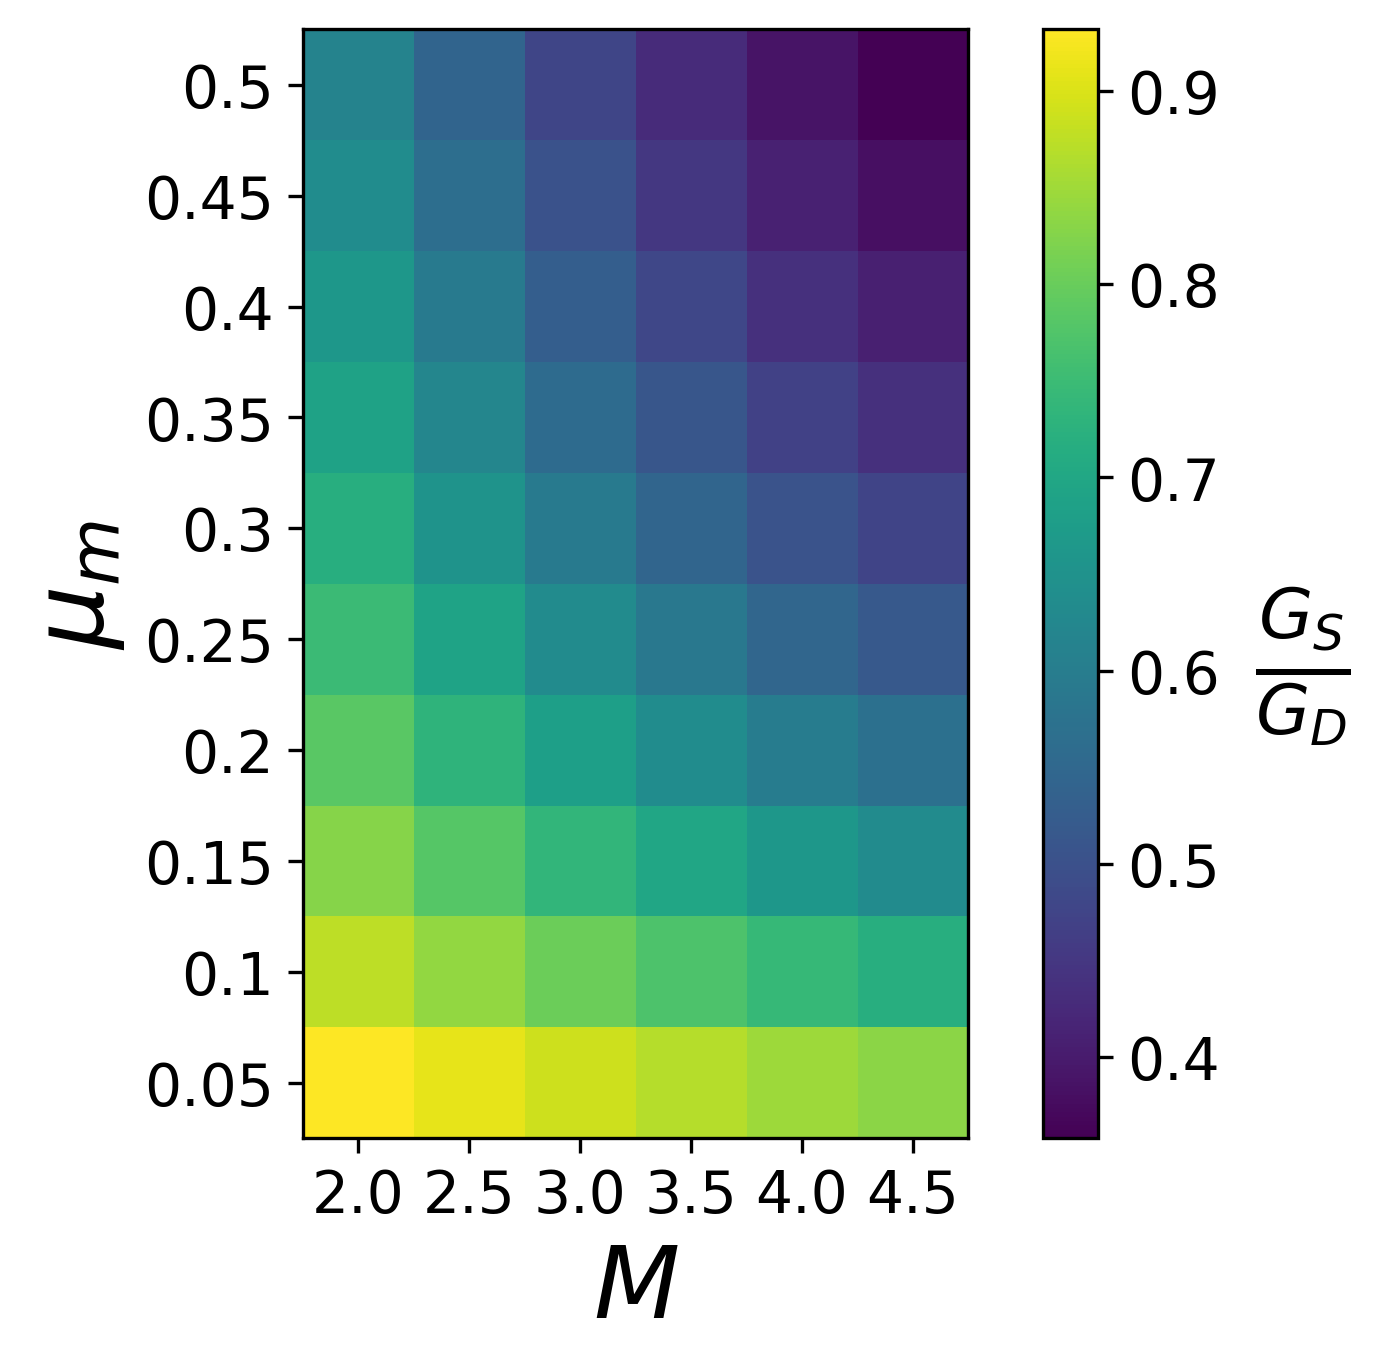
\includegraphics[width=0.45\linewidth]{chapters/DoubleNetworkFracture/Extra Images/StiffnessRatio.png}
    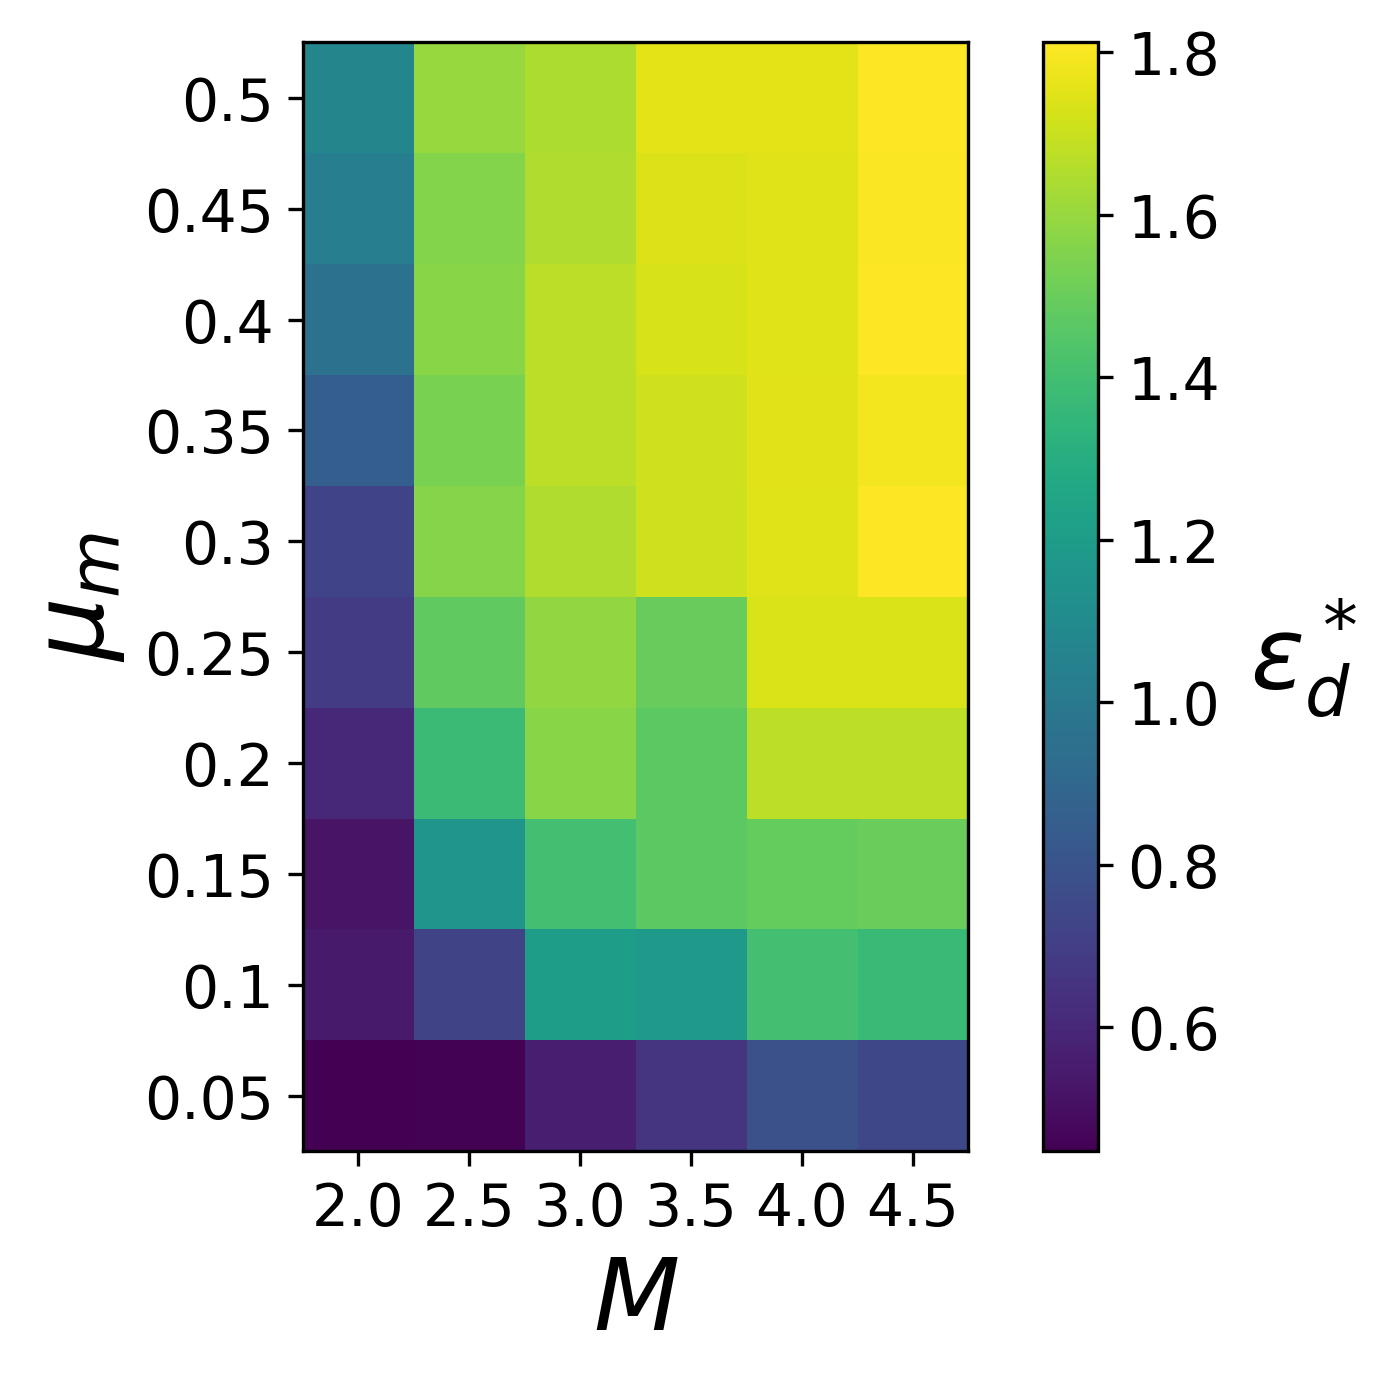
\includegraphics[width=0.45\linewidth]{chapters/DoubleNetworkFracture/Extra Images/Fail.png}
    \caption{Caption}
\end{figure}